%=======================================================
%	PACKAGES AND THEMES
%=======================================================
\documentclass[8pt]{beamer}
\mode<presentation> {
\usepackage{etex}
\usetheme{Boadilla}
\definecolor{navyblue}{rgb}{0.0, 0.0, 0.5}
\definecolor{dkgreen}{rgb}{0,0.6,0}
\definecolor{gray}{RGB}{64, 64, 64}
\definecolor{mauve}{rgb}{0.58,0,0.82}
\usecolortheme[named = navyblue]{structure}
\setbeamercolor{normal text}{fg = gray}
\setbeamercolor{frametitle}{fg = white, bg = navyblue}
\setbeamerfont{framesubtitle}{size = \normalsize}
\setbeamerfont{caption}{size=\footnotesize}
\setbeamercolor{page number in head/foot}{fg = gray}
\setbeamertemplate{footline}%[frame number]
}


\usepackage{graphicx} % Allows including images
\usepackage{booktabs} % Allows the use of \toprule, \midrule and \bottomrule in tables
\usepackage{multicol}
\usepackage[export]{adjustbox}
\usepackage{colortbl}
\usepackage{graphicx} 

\usepackage{tikz}
\usepackage{fancybox}
\usepackage[absolute, overlay]{textpos}
\usepackage{multirow}
\usepackage{siunitx}
\usepackage{tcolorbox}


\usepackage{tikz}
\usepackage{calc}
\newlength{\outerradius}
\newlength{\innerradius}
\setlength{\outerradius}{0.50cm}
\setlength{\innerradius}{0.35cm}

\usepackage{listings}
\lstset{numbers=left,
	numberstyle=\tiny,
	numbersep=5pt,
	breaklines=true,
	showstringspaces=false,
	frame=l ,
	xleftmargin=15pt,
	xrightmargin=15pt,
	basicstyle=\ttfamily\scriptsize,
	stepnumber=1,
	keywordstyle=\color{blue},          % keyword style
  	commentstyle=\color{dkgreen},       % comment style
  	stringstyle=\color{mauve}         % string literal style
}
%Sprache Festelegen
\lstset{language=R}


%=======================================================
%	TITLE PAGE
%=======================================================

\title{\textbf{Network Models}}

\author{Dr Daniele Rotolo}

\institute
{
SPRU (Science Policy Research Unit) \\
Business School\\
University of Sussex \\

\medskip

\medskip

\medskip

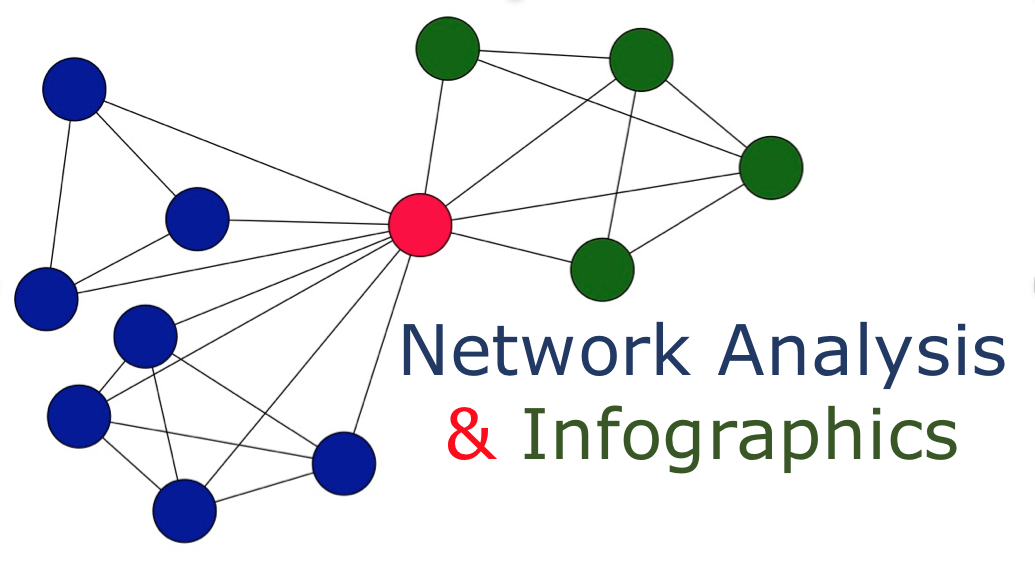
\includegraphics[width=2.5cm]{../_shared_pics/logo}

\medskip

\textit{{\color{dkgreen}{Week 8}}}\\
}


\date{} % Date, can be changed to a custom date

\begin{document}

\begin{frame}
\titlepage % Print the title page as the first slide

\begin{textblock*}{10pt}(0pt, 0.9\textheight)

\includegraphics[width=4cm]{../_shared_pics/SPRU.png}
\end{textblock*}

\end{frame}


%=======================================================
%	Learning outcomes
%=======================================================

\begin{frame}
\frametitle{Learning Outcomes}

\centering
\footnotesize
\begin{tabular}{lp{5.5cm}l}
\toprule
\multicolumn{2}{l}{\textbf{Learning outcome}} & \textbf{Assessment mode}\\
\hline
\\
1 & 
Explain the concept of network and list the main network indicators & 
ESS\\
\\
\rowcolor{green!20}2 & 
Describe and apply the major techniques for the collection of network data and their statistical analysis & 
ESS, GPN + GWS\\
\\
3 & 
Identify the main characteristics of networks by means of network measures  & 
ESS, GPN + GWS\\
\\
4 &
Employ network analysis techniques to produce network data-based infographics & 
GPN + GWS\\
\\
\bottomrule
\multicolumn{3}{l}{Note: ESS: Essay; GPN: Group Presentation; GWS: Group Written Submission}\\
\end{tabular}

\end{frame}

%------------------------------------------------



%=======================================================
%	Intro slides
%=======================================================
\section*{Overview}
%------------------------------------------------

\begin{frame}
\frametitle{\insertsection}
\tableofcontents[hideallsubsections]
\end{frame}

%------------------------------------------------






%=======================================================
% Network analysis [recap]
%=======================================================
\section{Network analysis [recap]}
%------------------------------------------------

\bgroup
\setbeamercolor{background canvas}{bg = navyblue}
\begin{frame}[plain]{}
\begin{center}
\color{white}{\Huge\insertsection}
\end{center}
\end{frame}
\egroup

%------------------------------------------------


\begin{frame}
\frametitle{\insertsection}
\setbeamercovered{transparent}

{\color{blue}{Descriptive network analysis}}
    \begin{itemize}
    \item An observed network is analysed by means of measures
    \item {\color{blue}{Network-level}} measures
    \item {\color{blue}{Node-level}} measures
    \end{itemize}

\bigskip
	
{\color{blue}{Modelling and inference of networks}}
    \begin{itemize}
    \item {\color{blue}{Mathematical models}}\\
    Based on `simple' probabilist rules to capture specific mechanisms (e.g.\ Erd\'os-R\'enyi networks, `the rich get richer')		
    \item {\color{blue}{Statistical models}}\\ 
    The observed network is considered as one of the possible realisation of a process -- a model that aims to fit to the observed data is specified (e.g.\ explanatory power of certain variables)
    \end{itemize}


\end{frame}

%------------------------------------------------

\begin{frame}
\frametitle{\insertsection}
\framesubtitle{Descriptive network analysis}

\medskip
\medskip

\begin{columns}[t]
\column{.45\textwidth} 
{\color{blue}{Network-level}} measures
        \begin{itemize}
        \item Diameter
        \item APL
        \item Density
        \item Components
        \item Cutpoints and bridges
        \item Point/Line connectivity
        \item Cliques 
        \item Inclusiveness
        \item Reachable pairs 
        \item Transitivity
        \end{itemize}


\column{.45\textwidth}
{\color{blue}{Node-level}} measures
        \begin{itemize}
        \item Degree centrality
        \item Closeness centrality
        \item Betweenness centrality
        \item Bonacich's centrality
        \item Weighted centrality
        \item Brokerage roles
        \item Effective network size/efficiency
        \item Constraint
        \end{itemize}
            
\end{columns}

\end{frame}

%------------------------------------------------

\begin{frame}
\frametitle{\insertsection}
\setbeamercovered{transparent}

{\color{blue}{Descriptive network analysis}}
    \begin{itemize}
    \item An observed network is analysed by means of measures
    \item {\color{blue}{Network-level}} measures
    \item {\color{blue}{Node-level}} measures
    \end{itemize}

\bigskip
	
{\color{blue}{Modelling and inference of networks}}
    \begin{itemize}
    \item {\color{blue}{Mathematical models}}\\
    Based on `simple' probabilist rules to capture specific mechanisms (e.g.\ Erd\'os-R\'enyi networks, `the rich get richer')		
    \item {\color{blue}{Statistical models}}\\ 
    The observed network is considered as one of the possible realisation of a process -- a model that aims to fit to the observed data is specified (e.g.\ explanatory power of certain variables)
    \end{itemize}


\end{frame}

%------------------------------------------------



%=======================================================
%	Network models
%=======================================================
\section{Modelling and inference of networks}

%------------------------------------------------

\bgroup
\setbeamercolor{background canvas}{bg = navyblue}
\begin{frame}[plain]{}
\begin{center}
\color{white}{\Huge\insertsection}
\end{center}
\end{frame}
\egroup

%------------------------------------------------


\begin{frame}
\frametitle{\insertsection}
\framesubtitle{Why do we need network models?}

\begin{itemize}
\item To {\color{blue}{generate networks}} with properties that we observe in the real world
\item To test the {\color{blue}{significance of certain characteristics}} in a given network (e.g.\ is the observed network expected?)
\item To identify which {\color{blue}{factors predict the formation of ties}}  (e.g.\ endogenous and exogenous factors)
\end{itemize}


\end{frame}

%------------------------------------------------

\begin{frame}
\frametitle{\insertsection}
\framesubtitle{Why do we need network models?}

\centering
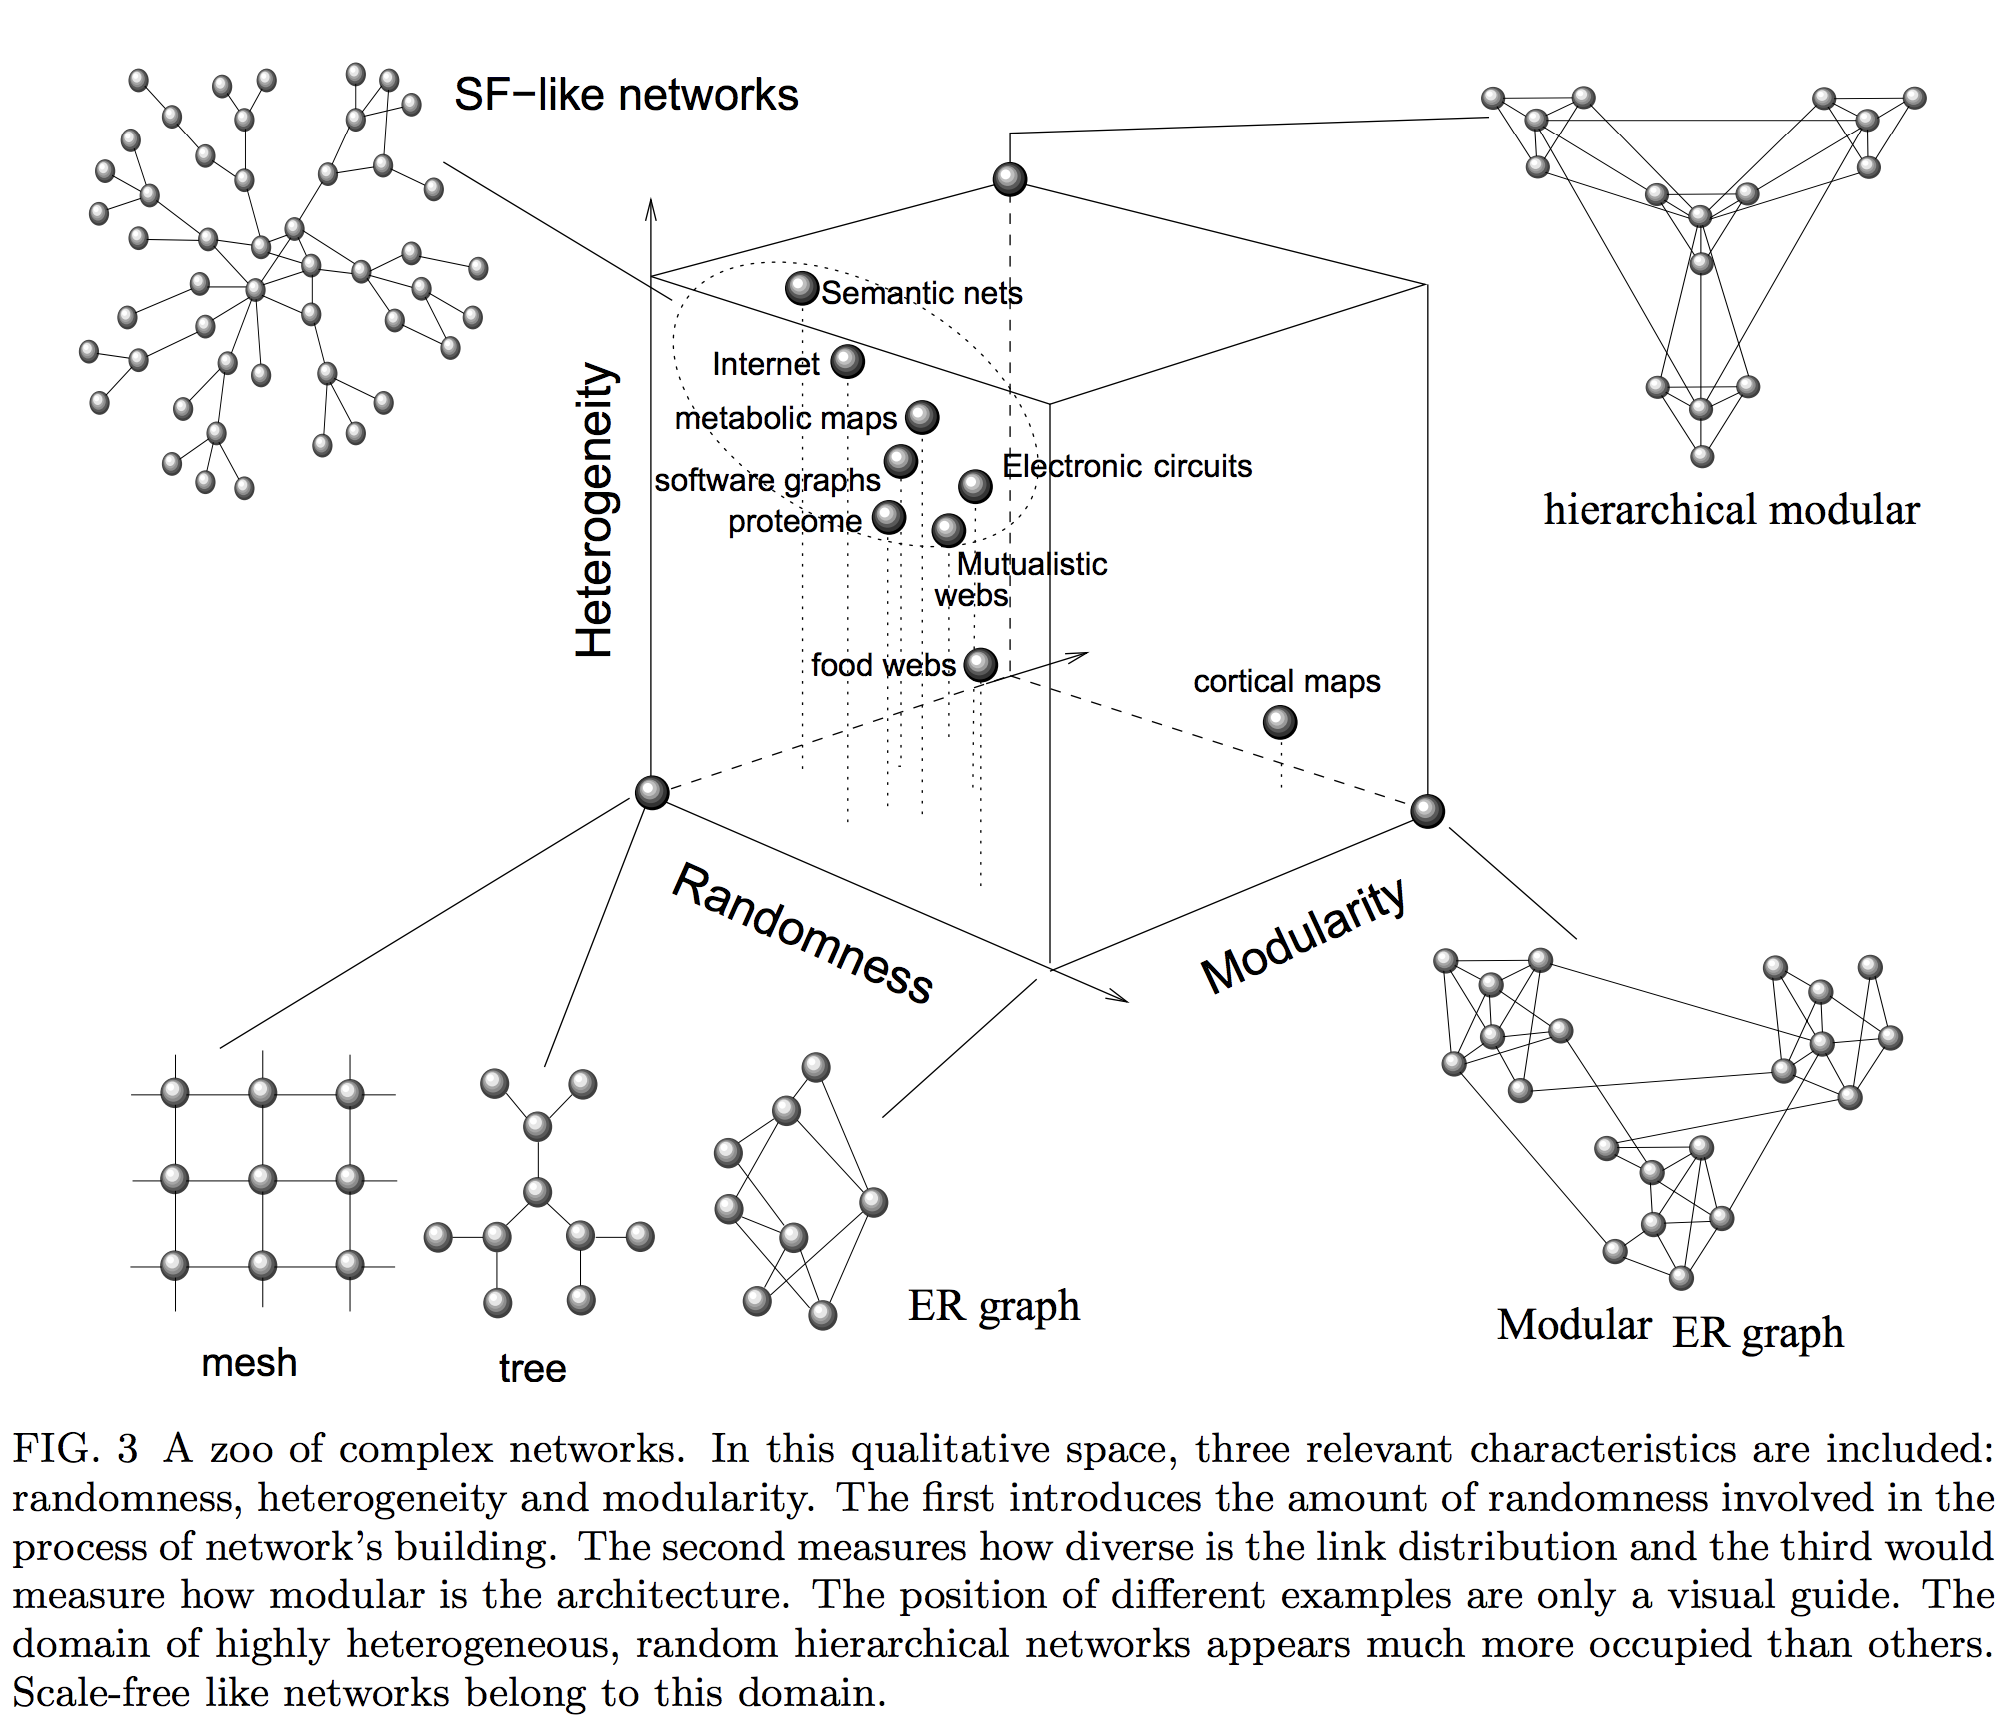
\includegraphics[width=0.7\textwidth]{network_map}\\
\tiny Source: \cite{Sole2004}

\end{frame}

%------------------------------------------------


\begin{frame}
\frametitle{\insertsection}
\framesubtitle{Why do we need network models?}

We can define a model for a network as a {\color{blue}{collection of networks}} $\mathbb{G}$ \cite{Kolaczyk2014}:

\begin{equation*}
\{\mathbb{P}_{\theta}(G), G \in \mathbb{G}: \theta \in \Theta\}
\end{equation*}

\begin{itemize}
\item $\mathbb{P}_{\theta}$ is the {\color{blue}{probability distribution}} of $\mathbb{G}$ --- its definition has a fundamental role in defining the model
\item $\theta$ is a {\color{blue}{vector of parameters}} the values of which range in $\Theta$
\end{itemize}

\end{frame}

%------------------------------------------------






%=======================================================
% Mathematical models
%=======================================================
\section{Mathematical models}

%------------------------------------------------

\bgroup
\setbeamercolor{background canvas}{bg = navyblue}
\begin{frame}[plain]{}
\begin{center}
\color{white}{\Huge\insertsection}
\end{center}
\end{frame}
\egroup

%------------------------------------------------

\begin{frame}
\frametitle{\insertsection}

\begin{itemize}
\item  {\color{blue}{Random graph models}} assume $\mathbb{P}_{\theta}(G)$ to be a uniform distribution
	\begin{itemize}
	\item {\color{blue}{Erd\'os-R\'enyi}} random graph model
	\item {\color{blue}{Bernoulli}} random graph model
	\item {\color{blue}{Generalised}} random graph models
	\end{itemize}

\medskip
\medskip

\item  {\color{blue}{Models based on mechanisms}} that aim to mimic certain properties observed in the real world (they are also called \textit{deterministic models})
	\begin{itemize}
	\item {\color{blue}{Small-worlds}} models
	\item {\color{blue}{Preferential attachment}} models
	\end{itemize}
	
\medskip
\medskip

\item Mathematical network models are often not capable to fitting observed data -- to address this issue {\color{blue}{statistical network models}} are used

\end{itemize}
\end{frame}

%------------------------------------------------

\begin{frame}
\frametitle{\insertsection}
\framesubtitle{Erd\'os-R\'enyi random graph model}

In the case of the {\color{blue}{Erd\'os-R\'enyi}} random graph model networks with $N$ nodes and $E$ edges are equally likely


\begin{equation*}
\mathbb{P}_{\theta}(G)={\binom{N_{G}}{E}}^{-1}
\end{equation*}

\begin{itemize}
\item $N$, number of nodes
\item $E$, number of edges
\item $\binom{N_{G}}{E}$ are all possible networks of $N$ nodes and $E$ edges (i.e.\ permutations)
\item $N_{G}= \binom{N}{2}$
\item binomial coefficient: $\binom{n}{k}=\frac{n!}{k!(n-k)!}$
\item factorial: $n!=n\times(n-1)\times(n-2)\times\ldots\times1$
\end{itemize}


\end{frame}

%------------------------------------------------

\begin{frame}
\frametitle{\insertsection}
\framesubtitle{Erd\'os-R\'enyi random graph model}

Example of a random network of $3$ nodes and $1$ edge, $G(3,1)$

\medskip

\centering
\onslide<2->{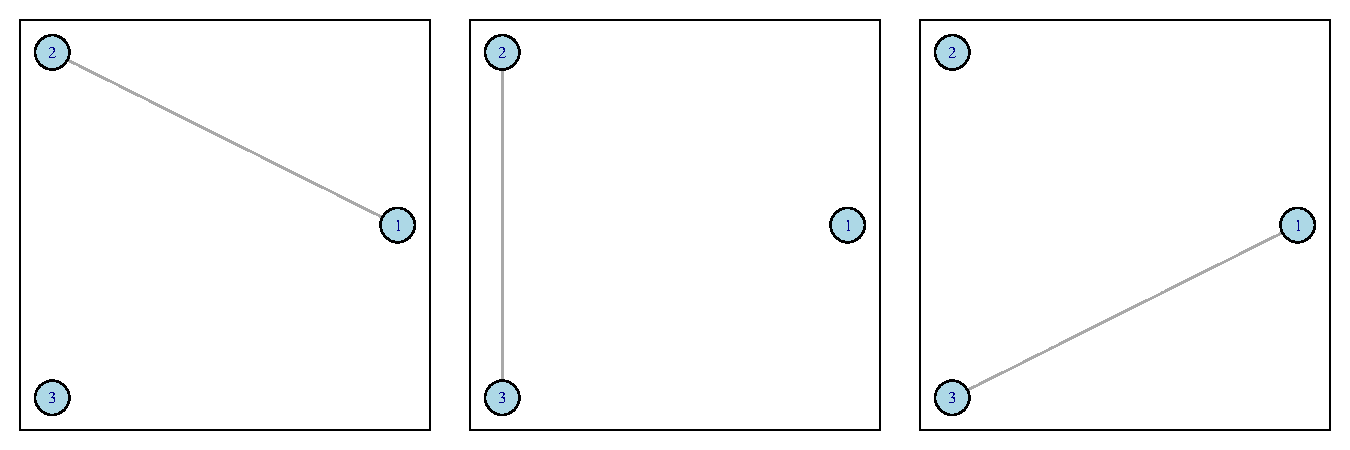
\includegraphics[width=0.9\textwidth]{erdos_3_1}}

\begin{enumerate}[<+(3)->]
\item $\mathbb{P}_{\theta}(G)={\binom{N_{G}}{E}}^{-1}$
\item $N_{G}= \binom{N}{2} = \binom{3}{2} = \frac{3!}{2!(3-2)!}=\frac{3\times2\times1}{(2\times1)\times(1)}=3$
\item $\binom{N_{G}}{E} = \binom{3}{1} = \frac{3!}{1!(3-1)!}=\frac{3\times2\times1}{(1)\times(2\times1)}=3$
\item $3$ possible permutations of $G(3,1)$
\item The probability of observing each network is ${\binom{N_{G}}{E}}^{-1}=\frac{1}{3} = 0.33$
\end{enumerate}

\end{frame}

%------------------------------------------------

\begin{frame}
\frametitle{\insertsection}
\framesubtitle{Erd\'os-R\'enyi random graph model}

Example of a random network of $4$ nodes and $1$ edge, $G(4,1)$

\begin{enumerate}
\item $\mathbb{P}_{\theta}(G)={\binom{N_{G}}{E}}^{-1}$
\item $N_{G}= \binom{N}{2} = \binom{4}{2} = \frac{4!}{2!(4-2)!}=\frac{4\times3\times2\times1}{(2\times1)\times(2\times1)}=6$
\item $\binom{N_{G}}{E} = \binom{6}{1} = \frac{6!}{1!(6-1)!}=\frac{6\times5\times4\times3\times2\times1}{(1)\times(5\times4\times3\times2\times1)}=6$
\item $6$ possible permutations of $G(6,1)$
\item The probability of observing each network is ${\binom{N_{G}}{E}}^{-1}=\frac{1}{6} = 0.17$
\end{enumerate}

\end{frame}

%------------------------------------------------

\begin{frame}
\frametitle{\insertsection}
\framesubtitle{Erd\'os-R\'enyi random graph model}

\centering
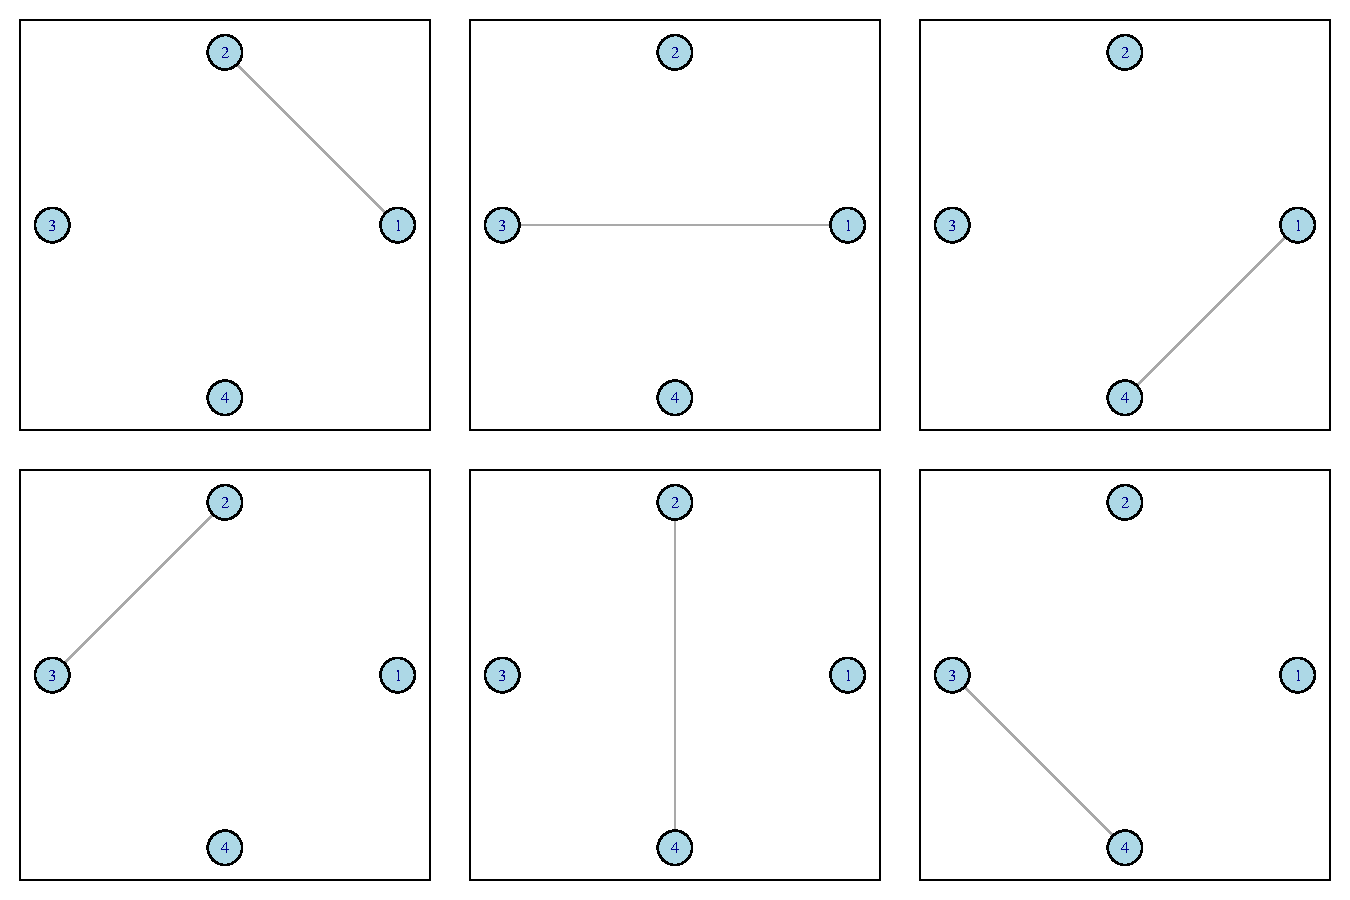
\includegraphics[width=0.9\textwidth]{erdos_4_1}

\end{frame}

%------------------------------------------------

\begin{frame}
\frametitle{\insertsection}
\framesubtitle{Erd\'os-R\'enyi random graph model}

The number of possible permutations can rapidly increase---for example let's consider a random network of $10$ nodes and $30$ edges, $G(10,30)$

\begin{enumerate}
\item $\mathbb{P}_{\theta}(G)={\binom{N_{G}}{E}}^{-1}$
\item $N_{G}= \binom{N}{2} = \binom{10}{2} = \frac{10!}{2!(10-2)!}= 45$
\item $\binom{N_{G}}{E} = \binom{45}{30} = \frac{45!}{30!(45-30)!}=344,867,425,584$
\item About $345$ billion of possible permutations of $G(10,30)$
\item The probability of observing each network is ${\binom{N_{G}}{E}}^{-1}=\frac{1}{344,867,425,584} = 2.9\times10^-12$
\end{enumerate}

\end{frame}

%------------------------------------------------

\begin{frame}
\frametitle{\insertsection}
\framesubtitle{Bernoulli random graph models}

The {\color{blue}{Bernoulli}} random graph model considers all graphs of $N$ nodes that are generated by independently assigning ties to nodes with a probability $p\in(0,1)$---networks with no edges or fully connected are not likely outcomes, but they are possible

\begin{equation*}
\mathbb{P}_{\theta}(G)=p^E(1-p)^{N_{G}-E}
\end{equation*}

\begin{itemize}
\item $N$, number of nodes
\item $E$, number of edges
\item $N_{G}= \binom{N}{2}$
\item binomial coefficient: $\binom{n}{k}=\frac{n!}{k!(n-k)!}$
\item factorial: $n!=n\times(n-1)\times(n-2)\times\ldots\times1$
\end{itemize}

\end{frame}

%------------------------------------------------

\begin{frame}
\frametitle{\insertsection}
\framesubtitle{Bernoulli random graph models}

Example of a random network of $10$ nodes and ties between nodes with $p=0.20$

\centering
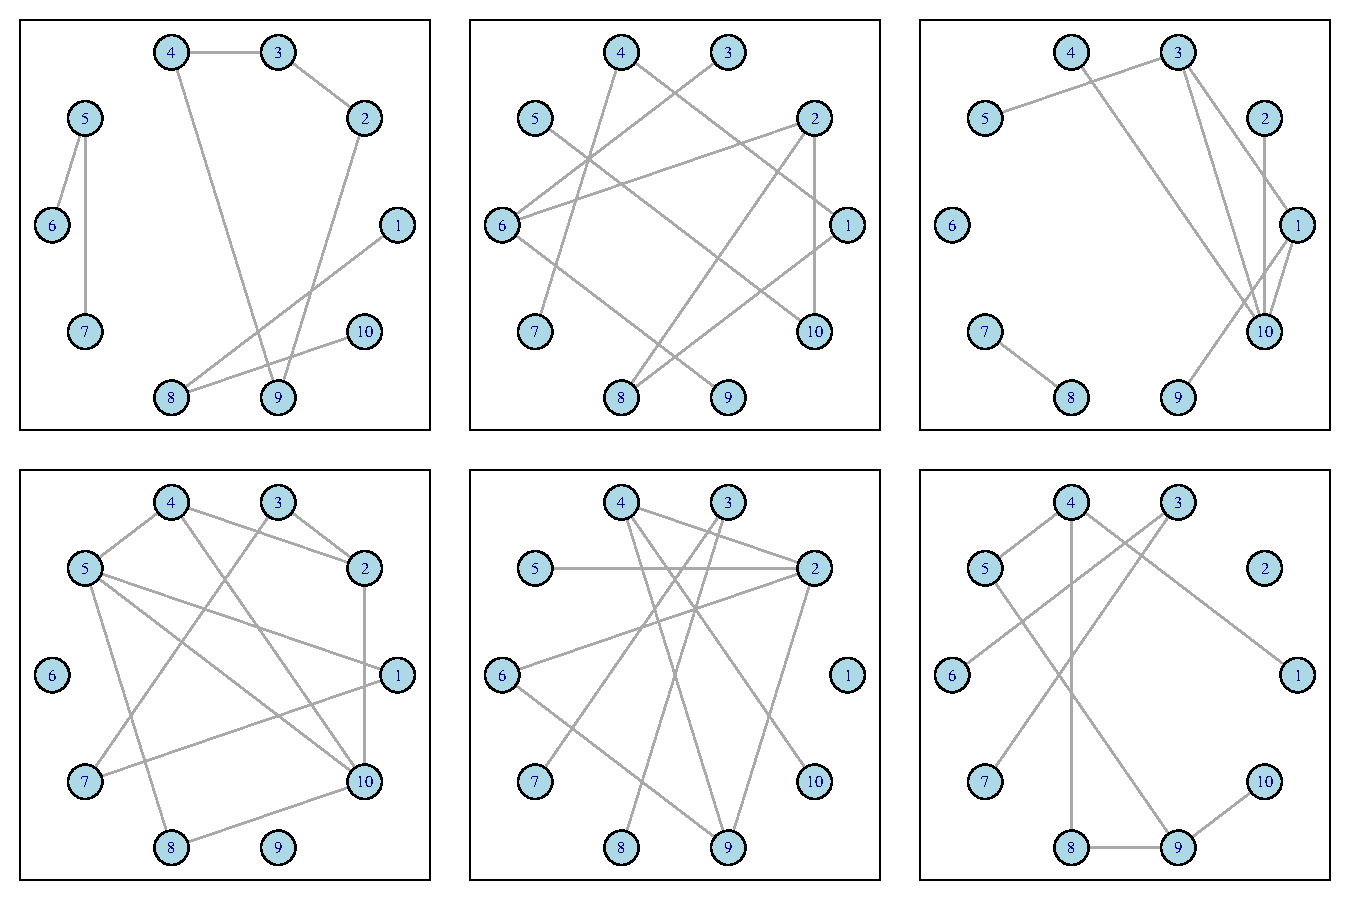
\includegraphics[width=0.8\textwidth]{bernoulli}

\end{frame}

%------------------------------------------------

\begin{frame}
\frametitle{\insertsection}
\framesubtitle{Bernoulli random graph models}

\begin{columns}[c]

\column{.45\textwidth} 
\begin{minipage}[c][.5\textheight][c]{\linewidth}


\begin{itemize}
\item Network generated by using Bernoulli random graph models are likely to have a {\color{blue}{giant component}} when $p>1/N$
\item Erd\'os-R\'enyi and Bernoulli random graph models are equivalent for large $N$ and when $E \sim pN^2$
\end{itemize}
\end{minipage}	   


\column{.55\textwidth}
\begin{minipage}[c][.5\textheight][c]{\linewidth}
\centering
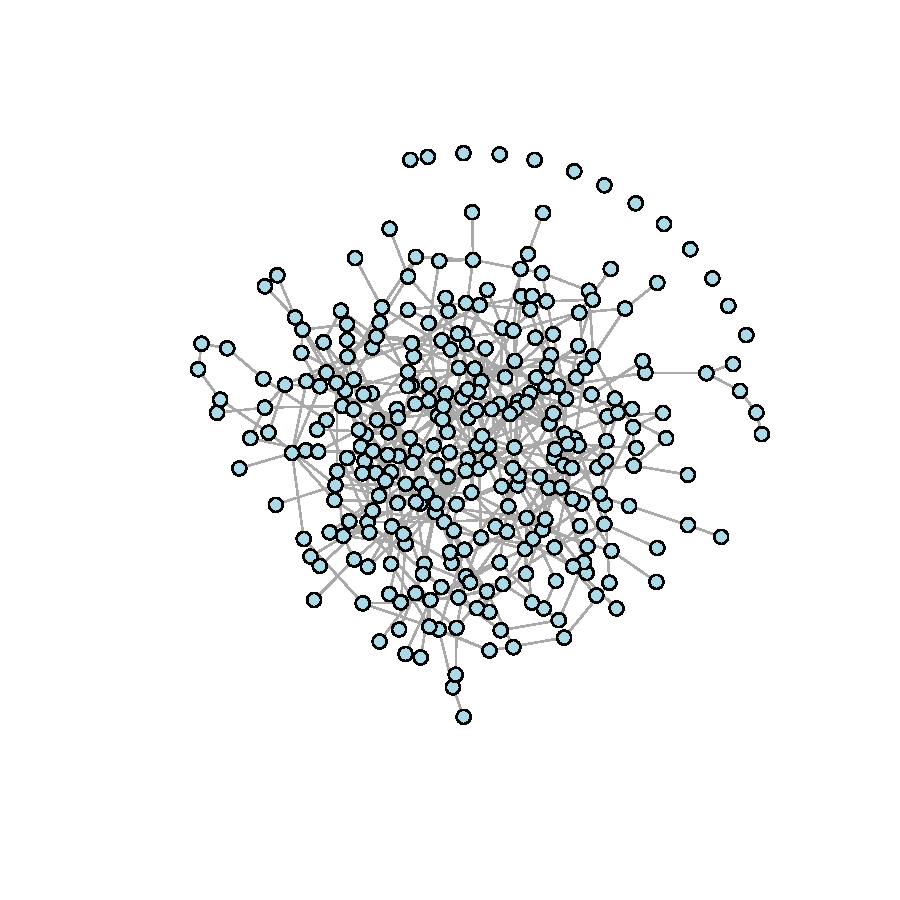
\includegraphics[height=0.8\textheight]{bernoulli_giant}
\end{minipage}

\end{columns}

\end{frame}

%------------------------------------------------

\begin{frame}
\frametitle{\insertsection}
\framesubtitle{Mathematical models: Erd\'os-R\'enyi and Bernoulli random graph models}

\centering
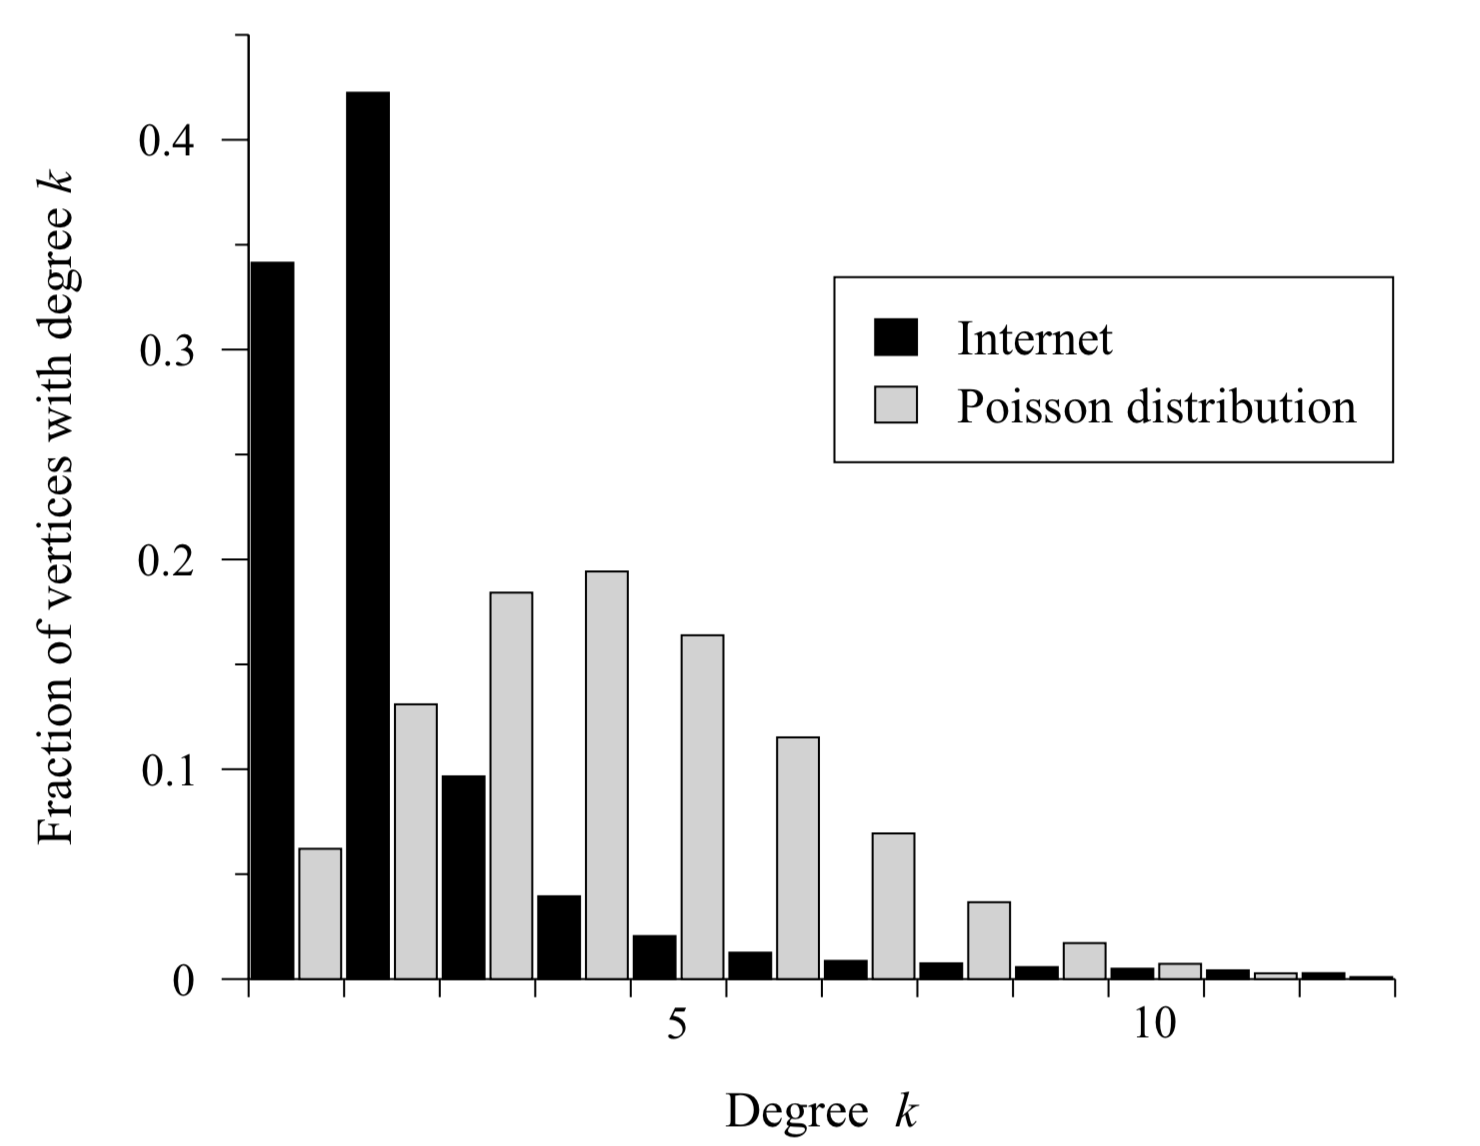
\includegraphics[height=0.8\textheight]{newman}\\
\tiny{Source: Distributions with the same averages of degree \cite{Newman2010}}

\end{frame}

%------------------------------------------------

\begin{frame}
\frametitle{\insertsection}
\framesubtitle{Mathematical models: Erd\'os-R\'enyi and Bernoulli random graph models}

\centering
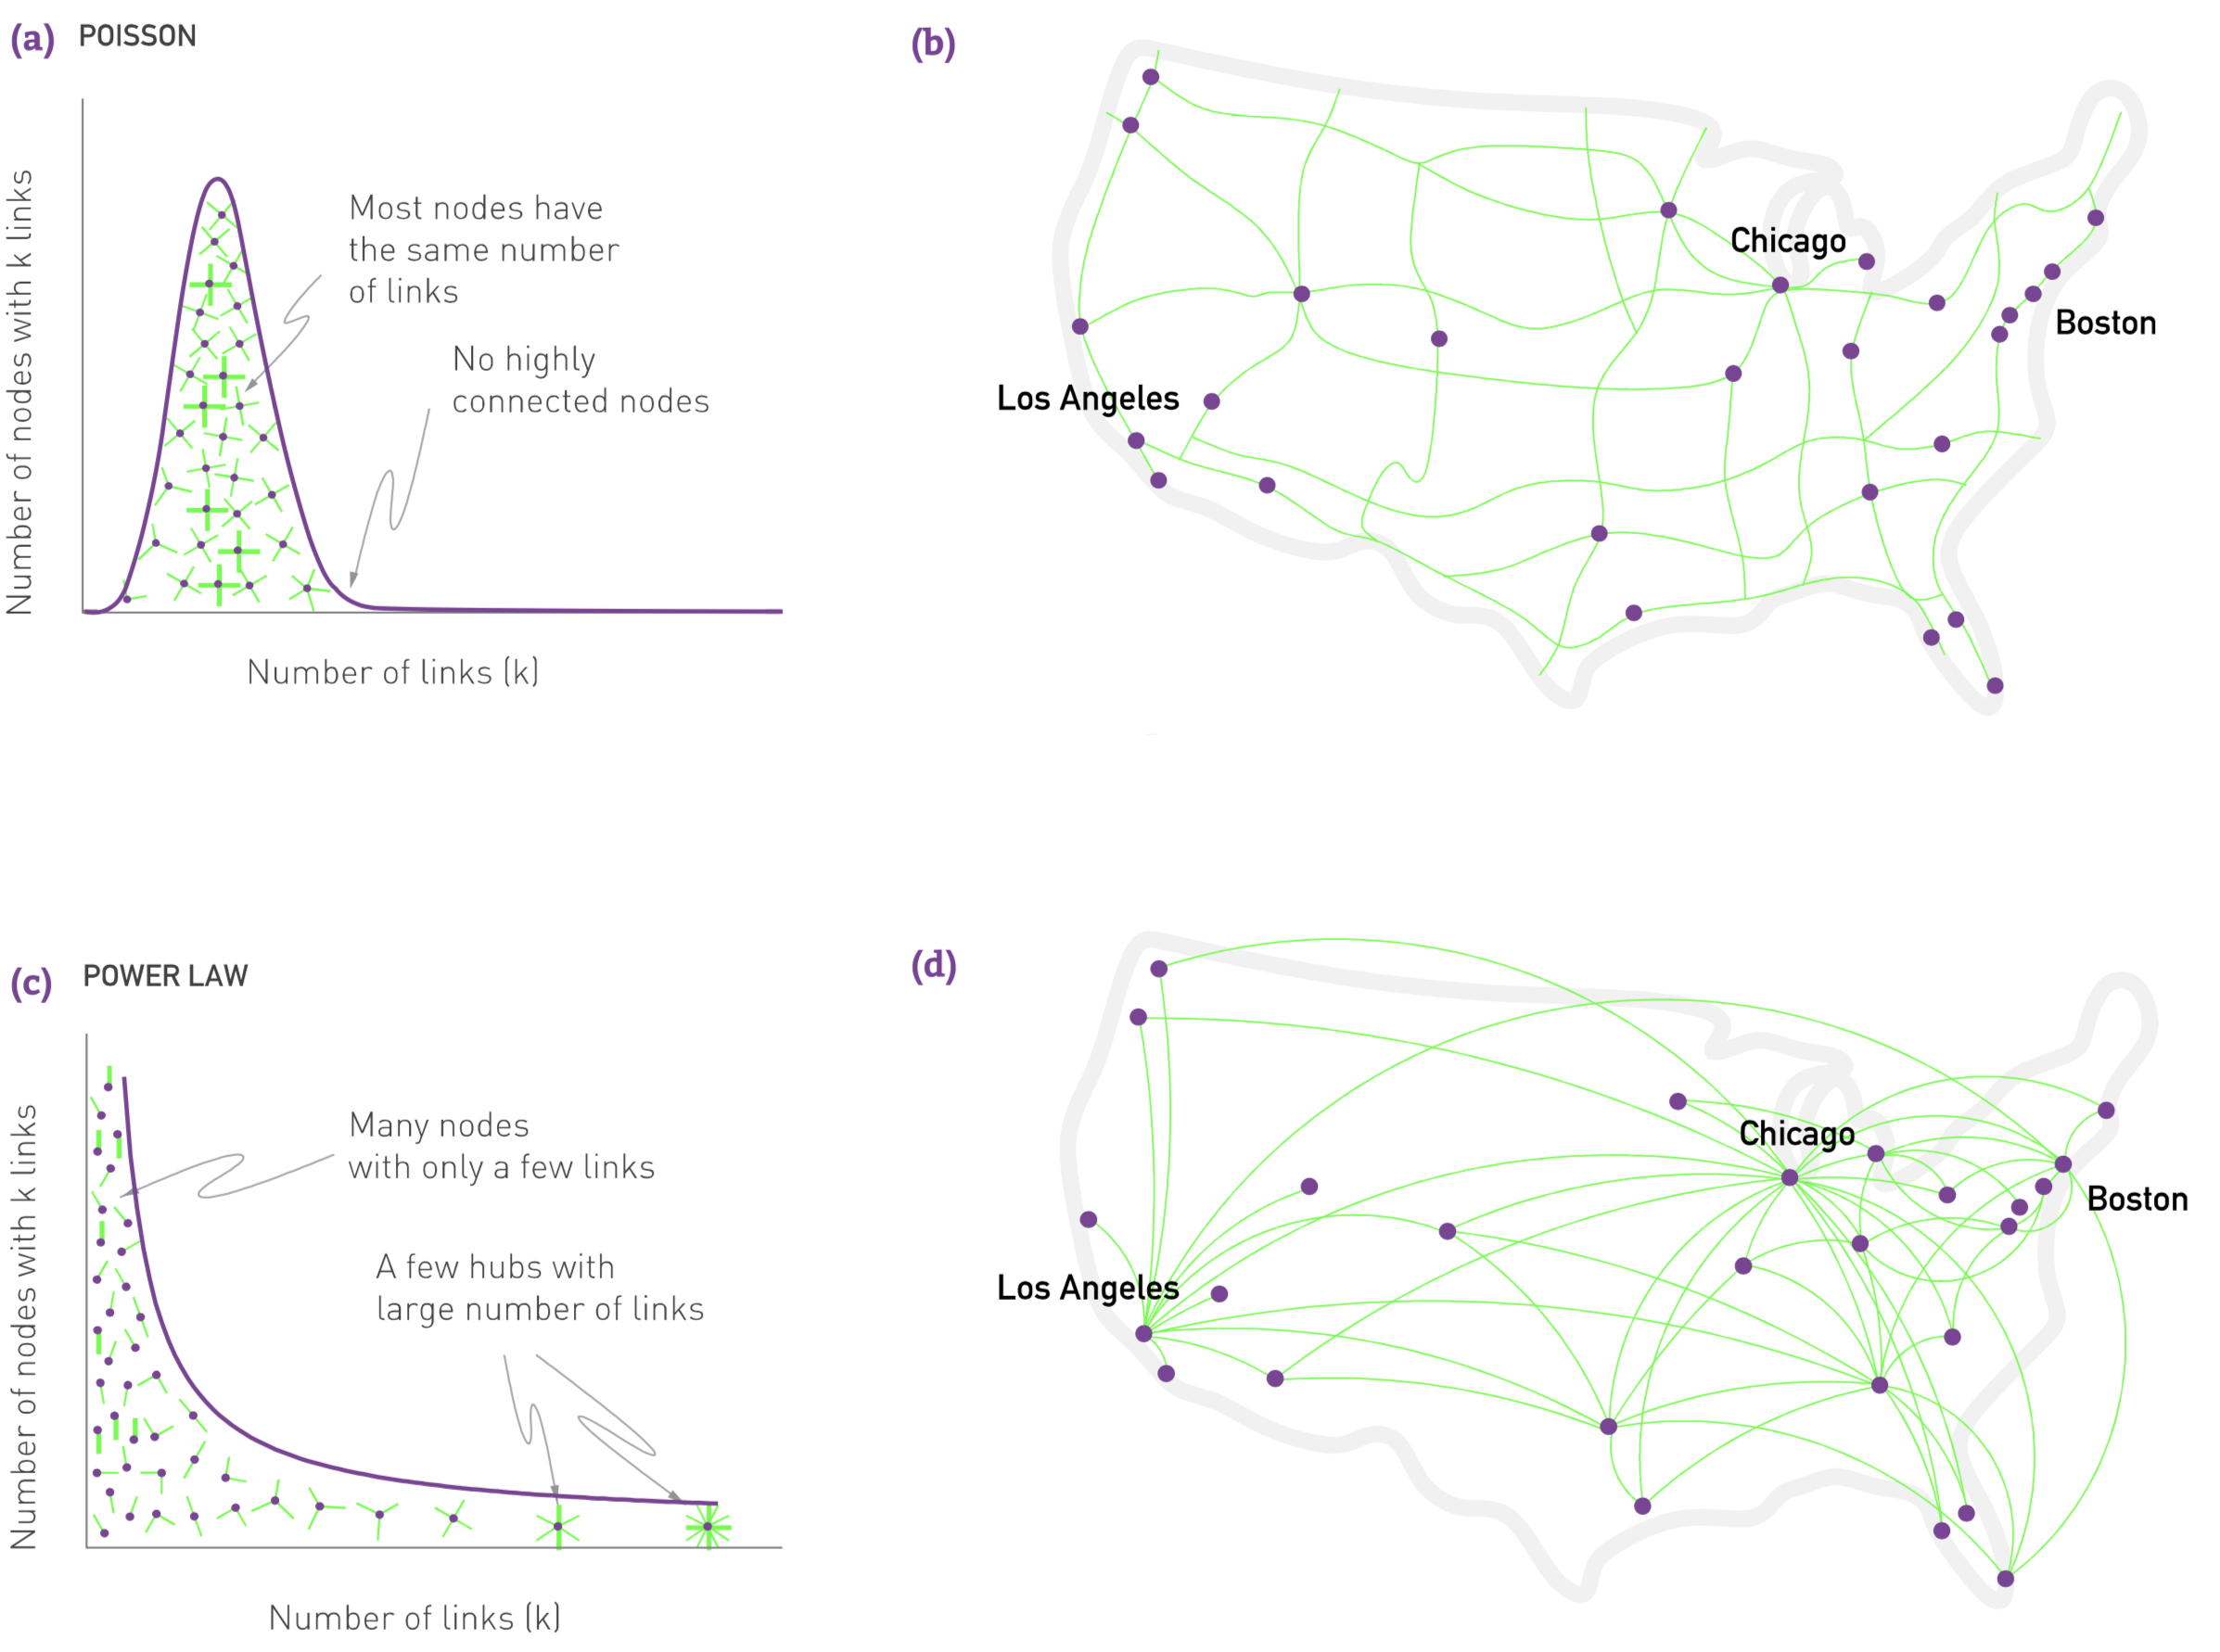
\includegraphics[height=0.8\textheight]{scale_free2}\\
\tiny{Source: Random networks (top, road connections) and scale-free networks (bottom, flight connections) \cite{Barabasi2016}}

\end{frame}

%------------------------------------------------

\begin{frame}
\frametitle{\insertsection}
\framesubtitle{Mathematical models: Generalised random graph models}

{\color{blue}{Generalised}} random graph model extends the Erd\'os-R\'enyi random graph model to a collection of graph of $N$ nodes that have certain properties
\begin{itemize}
	\item Two stubs are {\color{blue}{chosen uniformly at random}} and connected, with the number of stubs for a node equal to the defined degree of the node
	\item The sum of degree values must be even
	\item Networks do not appear with the same probability
	\item Example: $N=10$ and $d(2,2,2,2,2,4,4,4,4,4)$
\end{itemize}
	
\medskip

\centering
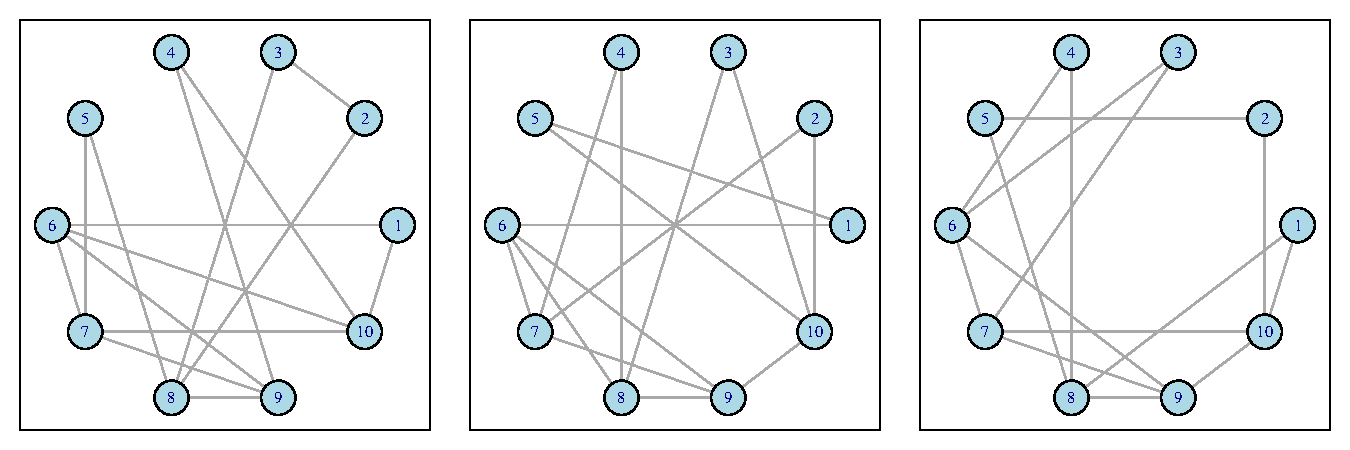
\includegraphics[width=0.9\textwidth]{generalised}

\end{frame}

%------------------------------------------------

\begin{frame}
\frametitle{\insertsection}
\framesubtitle{Mathematical models: Deterministic models}

Deterministic models attempts to generate two main {\color{blue}{characteristics that are observed in real networks}}, but that are not adequately reproduced by random graph models
\begin{itemize}
	\item Scale-free networks (i.e.\ degree distribution following a power law) \\ 
		  $\Rightarrow$ \textbf{Preferential attachment models}
	\item High levels of transitivity \\
		  $\Rightarrow$ \textbf{Small-world network}
\end{itemize}

\end{frame}

%------------------------------------------------

\begin{frame}
\frametitle{\insertsection}
\framesubtitle{Models based on mechanisms: Preferential attachment models}

{\color{blue}{Preferential attachment models}}: ``the rich get richer'' (used to model accumulation effect in science) \cite{Barabasi1999}

\begin{enumerate}
\item Network at $t=0$
\item The network is modified at $t=1$ by adding a node $j$ with a degree of $m>0$
\item The probability that each edge of the new node is attached to an existing node is proportional to the degree of the existing node: $\frac{C_D(n_i)}{\sum_k{C_D(n_k)}}$
\item This model is likely to generate {\color{blue}{hubs}}, i.e.\ nodes with high degree
\end{enumerate}

\end{frame}

%Note=========
%For $t \rightarrow \infty $, the degree distribution assume the form of a power law ($\alpha=3$)
%=============

%------------------------------------------------

\begin{frame}
\frametitle{\insertsection}
\framesubtitle{Models based on mechanisms: Preferential attachment models}

\begin{columns}
\column{.50\textwidth}
\centering
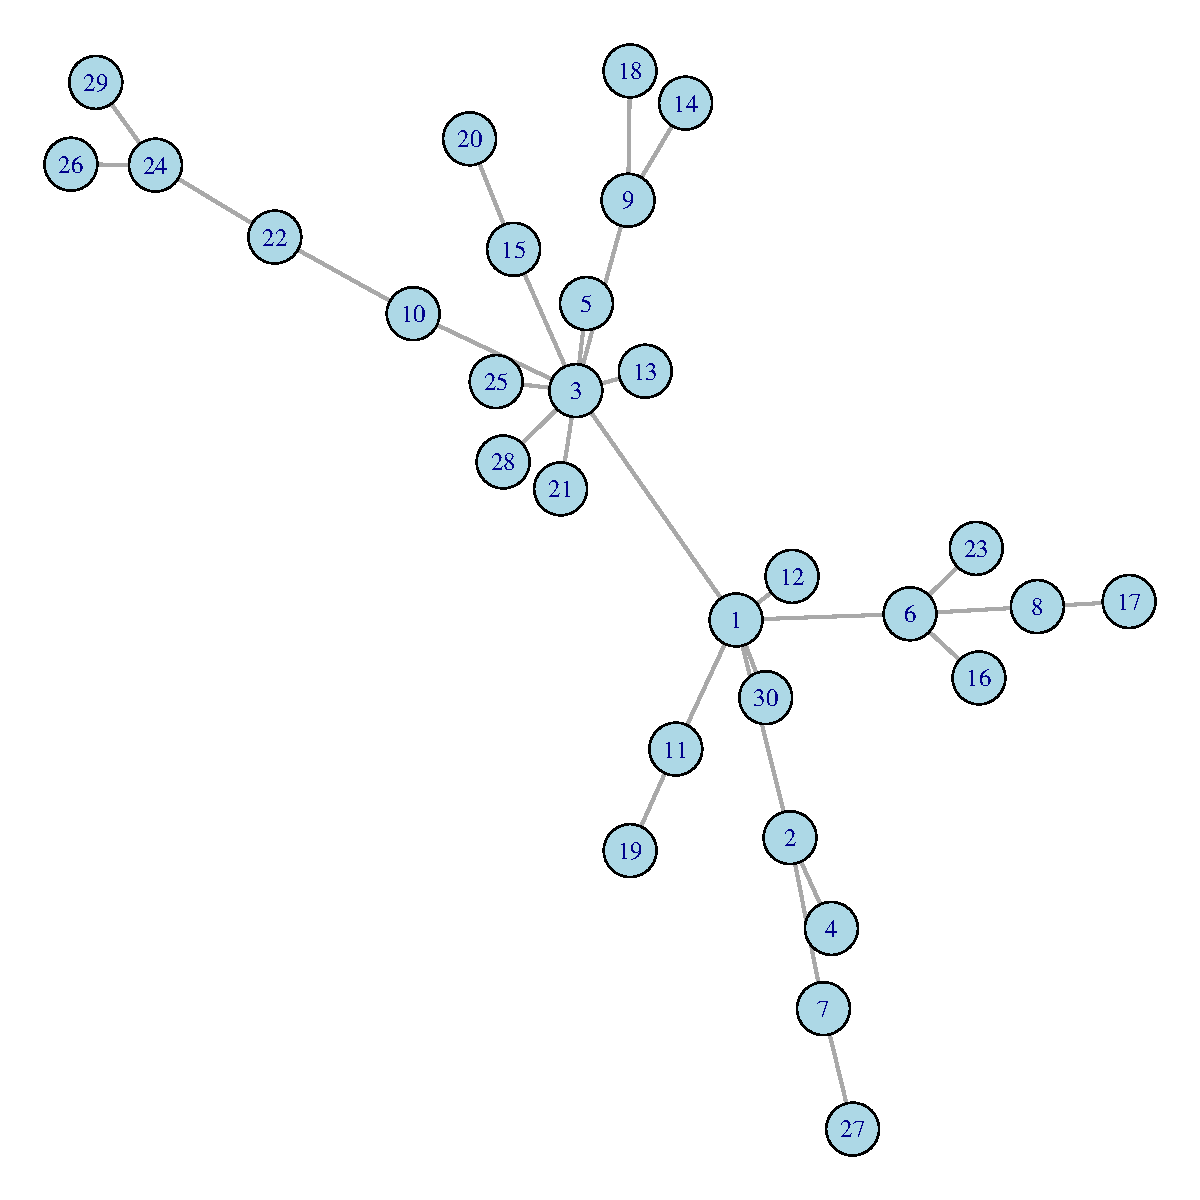
\includegraphics[width=\textwidth]{barabasi1}

\column{.50\textwidth}
\centering 
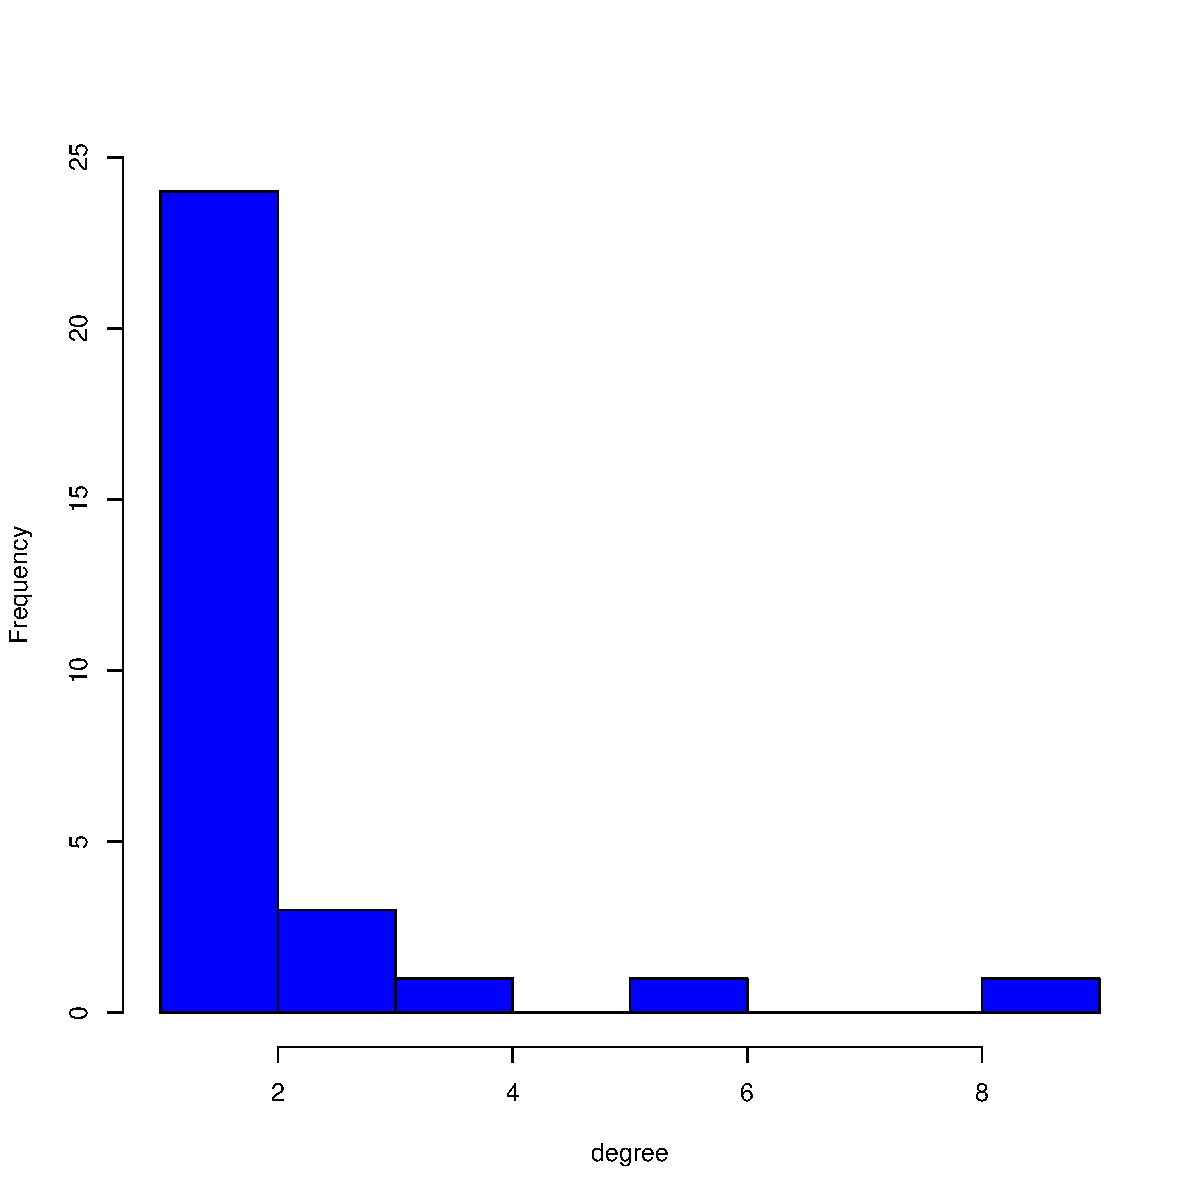
\includegraphics[width=\textwidth]{barabasi2}

\end{columns}

\end{frame}
%------------------------------------------------

\begin{frame}
\frametitle{\insertsection}
\framesubtitle{Models based on mechanisms: Small-world models}

\begin{columns}
\column{.45\textwidth}
{\color{blue}{Small-world models}} generate networks with high clustering and small distances between nodes \cite{Watts1998} 

\begin{itemize}
\item Clustering coefficient (or transitivity): $C = \frac{\text{number of triangles x 3} }{\text{number of connected triples}}$
\item High clustering in relation to $c/N$
\item Many networks in the real world have these characteristics
\item `Six degree of separation'
\item Brain connectivity (neurons)
\item Power grids
\item ...
\item Specialisation and efficiency
\item Do not mimic scale-free networks
\end{itemize}

\column{.45\textwidth}
\centering
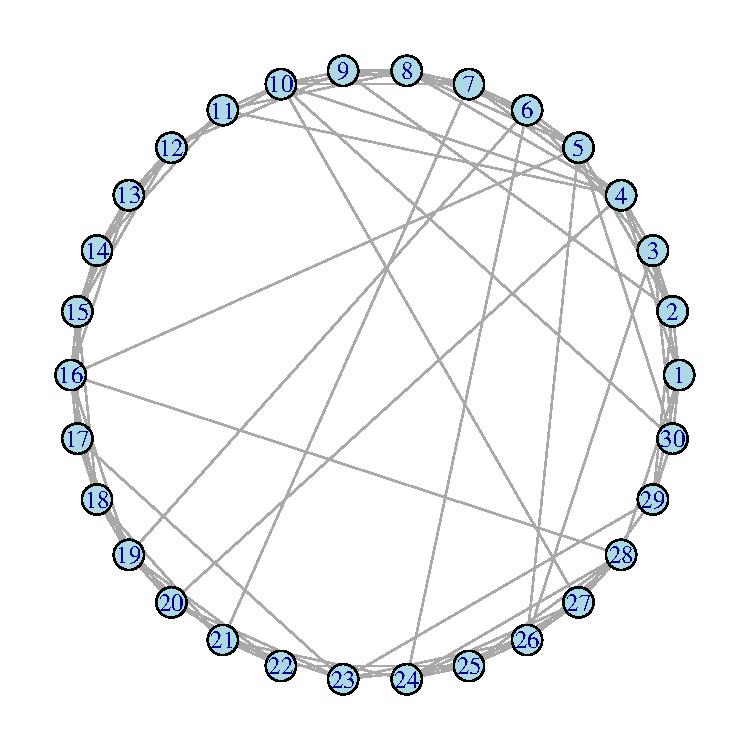
\includegraphics[width=0.8\textwidth]{sm} \\
\medskip
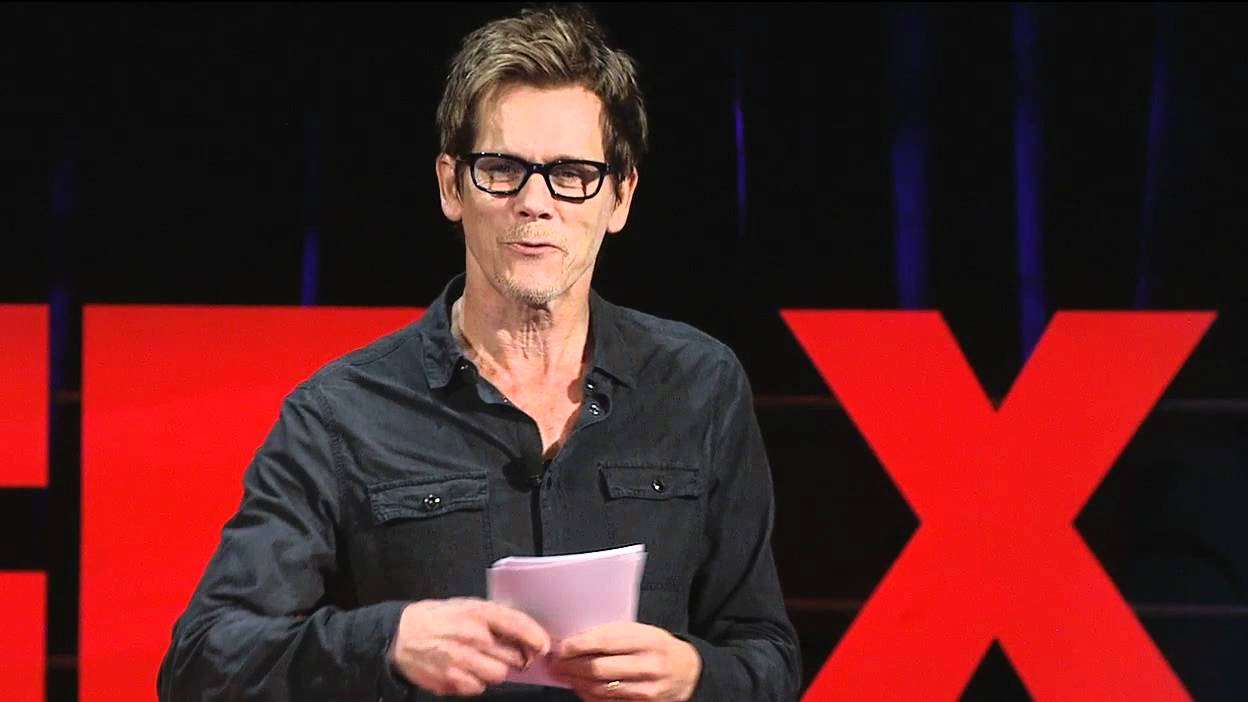
\includegraphics[width=4cm]{bacon}\\
\tiny{Source: Kevin Bacon's six degree of separation (\url{www.youtube.com/watch?v=n9u-TITxwoM})}
\end{columns}

\end{frame}

%------------------------------------------------

\begin{frame}
\frametitle{\insertsection}
\framesubtitle{Models based on mechanisms: Small-world models}

\begin{enumerate}
    \item Creation of a network of $N$ nodes with {\color{blue}{lattice structure}}: each node is connected to $r$ of its neighbours
    \item Each edge, independently and with probability $p$, is moved to be incident to another node, which is chosen uniformly (no loops and multi-edges)
 \end{enumerate}

\begin{columns}[t]

\column{.33\textwidth}
\centering
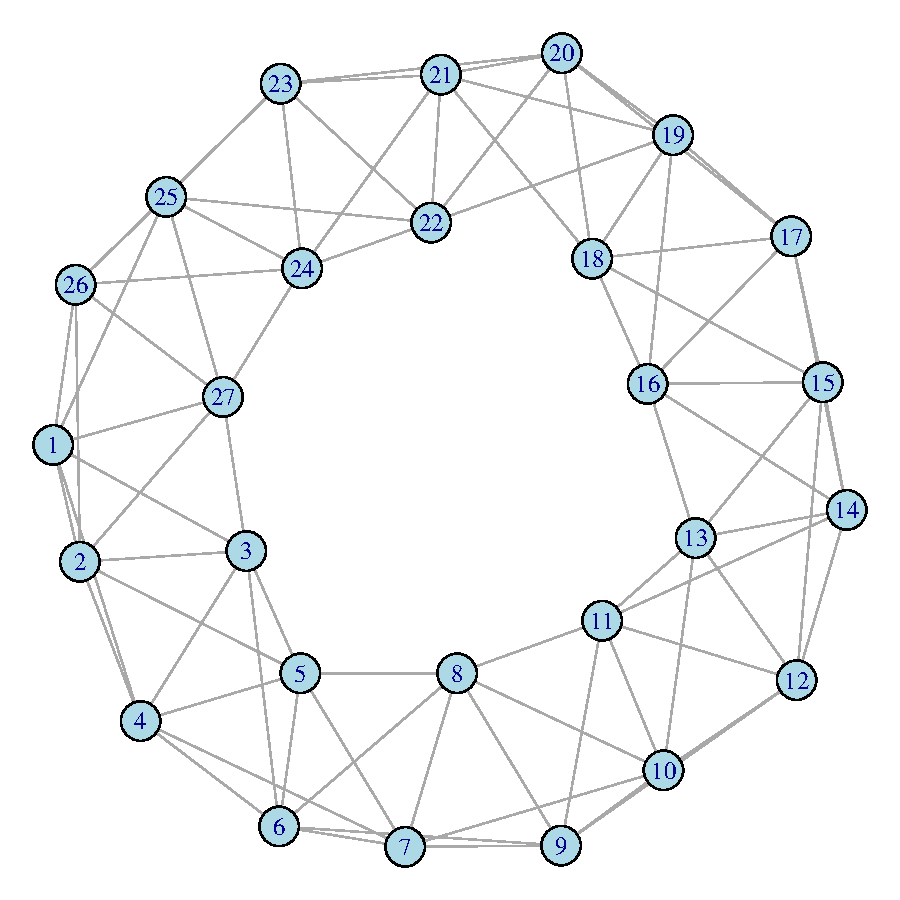
\includegraphics[width=3.5cm]{sm1}\\
\tiny{lattice structure\\
$N=27$, $r=3$}

\column{.33\textwidth}
\centering 
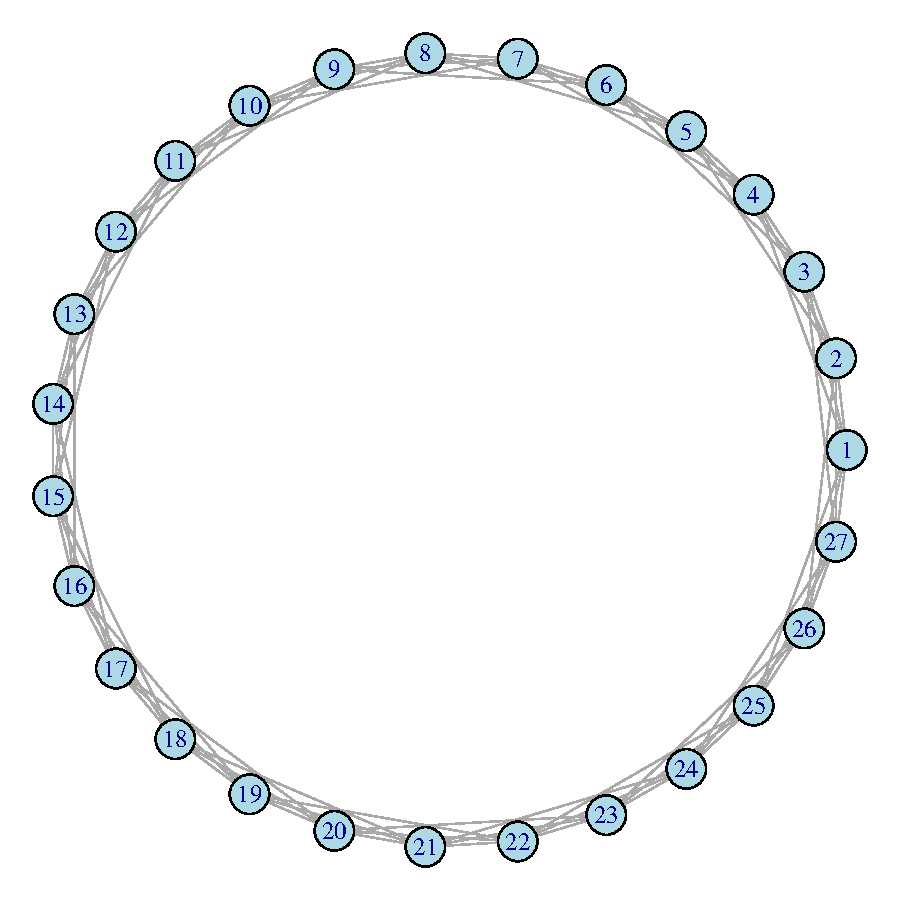
\includegraphics[width=3.5cm]{sm1_c}\\
\tiny{lattice structure (circle layout)\\
$N=27$, $r=3$}

\column{.33\textwidth}
\centering
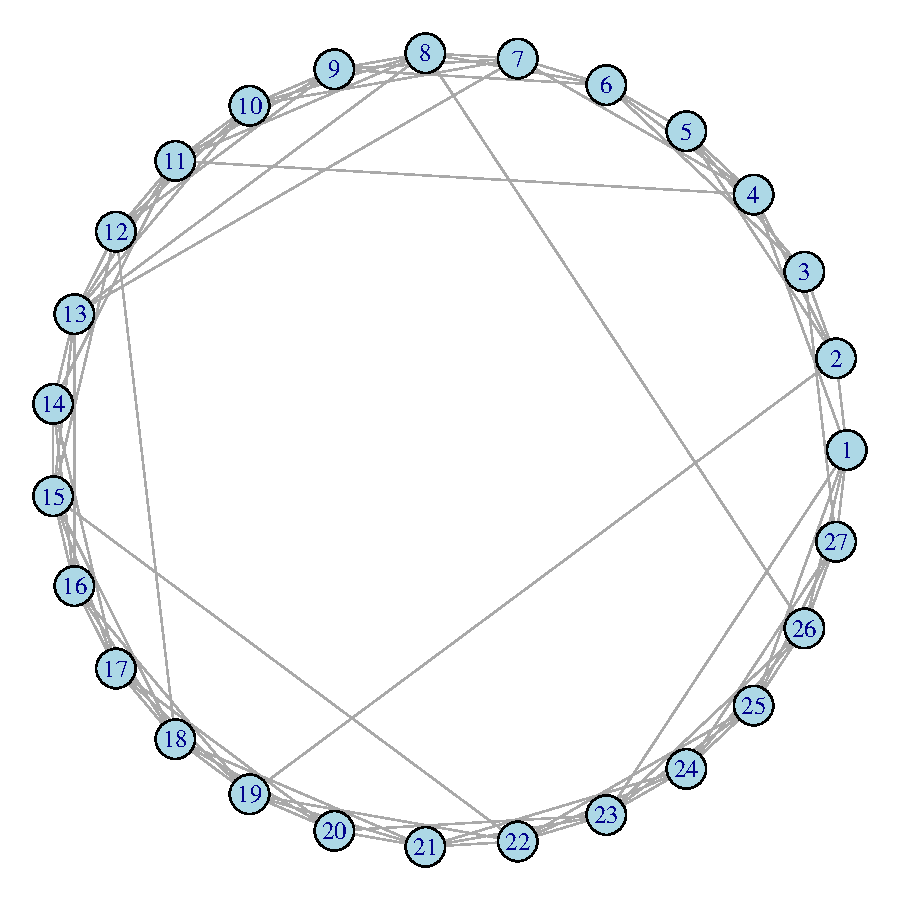
\includegraphics[width=3.5cm]{sm2}\\
\tiny{small-world network\\
 $N=27$, $r=3$, $p=0.1$}

\end{columns}

\end{frame}

%------------------------------------------------


%=======================================================
% Statistical network models
%=======================================================
\section{Statistical network models}
%------------------------------------------------

\bgroup
\setbeamercolor{background canvas}{bg = navyblue}
\begin{frame}[plain]{}
\begin{center}
\color{white}{\Huge\insertsection}
\end{center}
\end{frame}
\egroup

%------------------------------------------------

\begin{frame}
\frametitle{\insertsection}

Mathematical network models are often not capable to fitting observed data -- to address this issue {\color{blue}{statistical network models}} are used

\medskip

\begin{itemize}
\item {\color{blue}{Exponential Random Graph Models (ERGM)}} 
	\begin{itemize}
	\item Consider the {\color{blue}{presence/absence of a tie}} as the response variable
	\item The response variable is dependent on a number of {\color{blue}{endogenous}} (e.g.\ transitivity) and {\color{blue}{exogenous}} (e.g.\ attributes) characteristics \cite{Robins2007}
	\end{itemize}

\medskip
\medskip

\item{\color{blue}{Stochastic Actor-Oriented Models (SAOM)}}: The co-evolution of a network structure and attributes is modelled as a stochastic process \cite{Snijders2010}

\medskip
\medskip
  
\item {\color{blue}{Network Block Models}} model the propensity to establish a tie between two nodes as dependent on the `class' membership of the two nodes (e.g.\ nodes in the same class are more likely to establish a tie) \cite{Doreian1984}

\medskip
\medskip
\item ... new models every years (this is an emerging area) 
\end{itemize}


\end{frame}

%------------------------------------------------

\begin{frame}
\frametitle{\insertsection}
\framesubtitle{The key idea of ERGM}

Limitations of {\color{blue}{random graph models}} and {\color{blue}{the key idea of ERGM}}

\begin{itemize}

\item In the case of random graph models, we fix {\color{blue}{a network property}} in absolute values --- for example, the number of edges 

\item We then generate a (uniform) distribution of networks with such a property making assumption that {\color{blue}{ties between nodes occur at random}}

\item We are, however, excluding the possibility that the network we observe {\color{blue}{may have been different}} --- for example:
 	\begin{itemize}
 	\item we could have observed networks with a different number of edges
 	\item social forces may influence the formation of ties (e.g.\ preferential attachment)
 	\end{itemize}

\item A better approach would be: 
 \begin{itemize}
 \item to fix {\color{blue}{the average value of the network property}}, i.e.\ average number of edges
 \item to generate a {\color{blue}{distribution of networks}} where networks with a number of edges that is close to the desired value have higher probabilities than network with a lower/higher number of edges
 \end{itemize}
 
\end{itemize}

\end{frame}

%------------------------------------------------

\begin{frame}
\frametitle{\insertsection}
\framesubtitle{The key idea of ERGM}

\begin{itemize}

\item {\color{blue}{ERGM}} gives flexibility by fixing multiple network properties:
	\begin{itemize}
	\item Number of edges or mean degree
	\item Degree of individual vertices
	\item Number of triangles or clustering coefficient
	\item ...
	\end{itemize}

\item Physicists and statisticians have demonstrated that the exponential distribution is the {\color{blue}{`best choice'}} (minimum assumptions except for those imposed by the properties we select)

\item We do not enter into the details of the estimation 

\end{itemize}

\end{frame}

%------------------------------------------------

\begin{frame}
\frametitle{\insertsection}
\framesubtitle{The formulation of ERGM}

The {\color{blue}{general formulation}} of ERGM is reported below:

\begin{equation*}
\mathbb{P}_\theta({\mathbf{Y} = \mathbf{y}}) = \frac{e^{\sum_k \theta_k s_k(\mathbf{y})}}{\sum_y(e^{\sum_k \theta_k s_k(\mathbf{y})})}
\end{equation*}


\begin{itemize}
\item $\mathbf{Y}=\lbrack Y_{ij} \rbrack$, is the random adjacency matrix
\item $\mathbf{y}=\lbrack y_{ij} \rbrack$, is the particular realisation of $\mathbf{Y}$
\item $\theta$, vector of $k$ parameters to estimate 
\item $s_k(\mathbf{y})$, independent variables (endogenous and/or exogenous)
\item In few words
	\begin{itemize}
	\item The {\color{blue}{numerator}} is the probability of observing the specific network $\mathbf{y}$
	\item The {\color{blue}{denominator}} is the sum of all probabilities of the networks in the distribution (this is, in general, very difficult to estimate: simulation with Markov Chain Monte Carlo Maximum Likelihood Estimation, MCMCMLE)
	\end{itemize}
\end{itemize}
\end{frame}

%------------------------------------------------

\begin{frame}
\frametitle{\insertsection}
\framesubtitle{The formulation of ERGM}

\centering
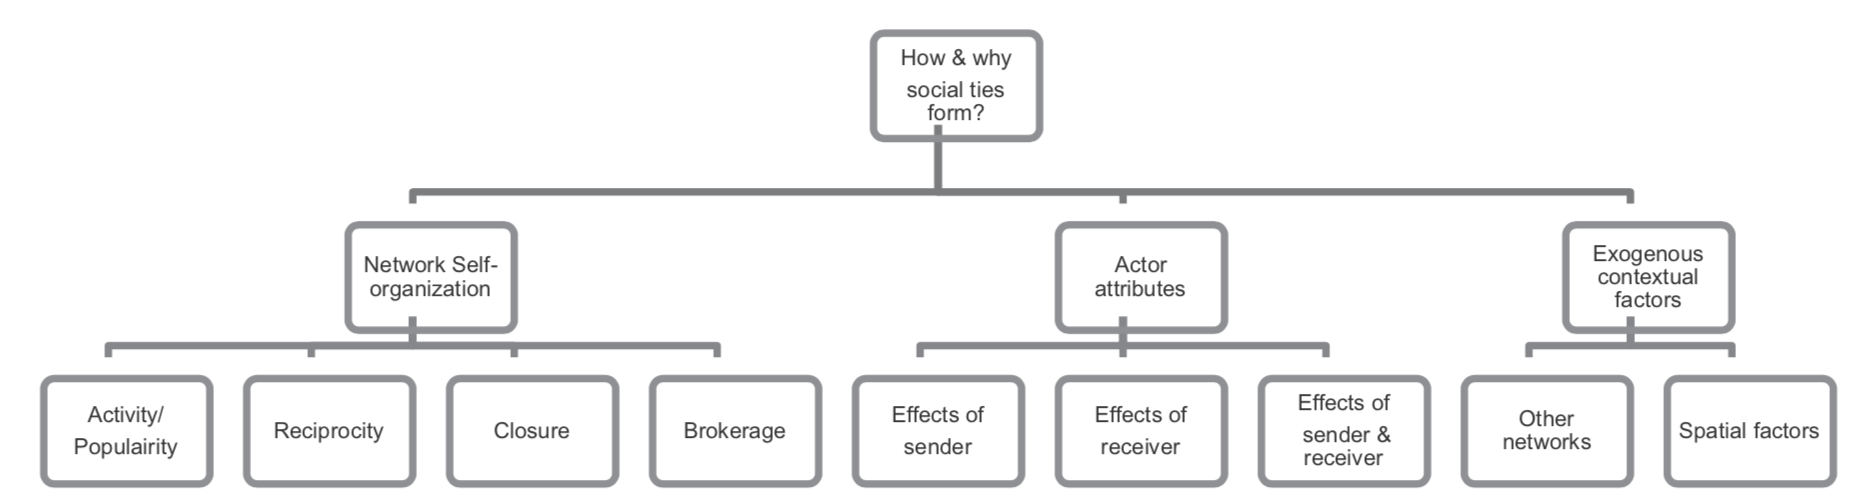
\includegraphics[width= \textwidth]{ergm_framework}\\
\tiny{Source: Selection of independent variables (endogenous and/or exogenous) \cite{Amati2018}}

\end{frame}

%------------------------------------------------

\begin{frame}
\frametitle{\insertsection}
\framesubtitle{The formulation of ERGM}

\centering
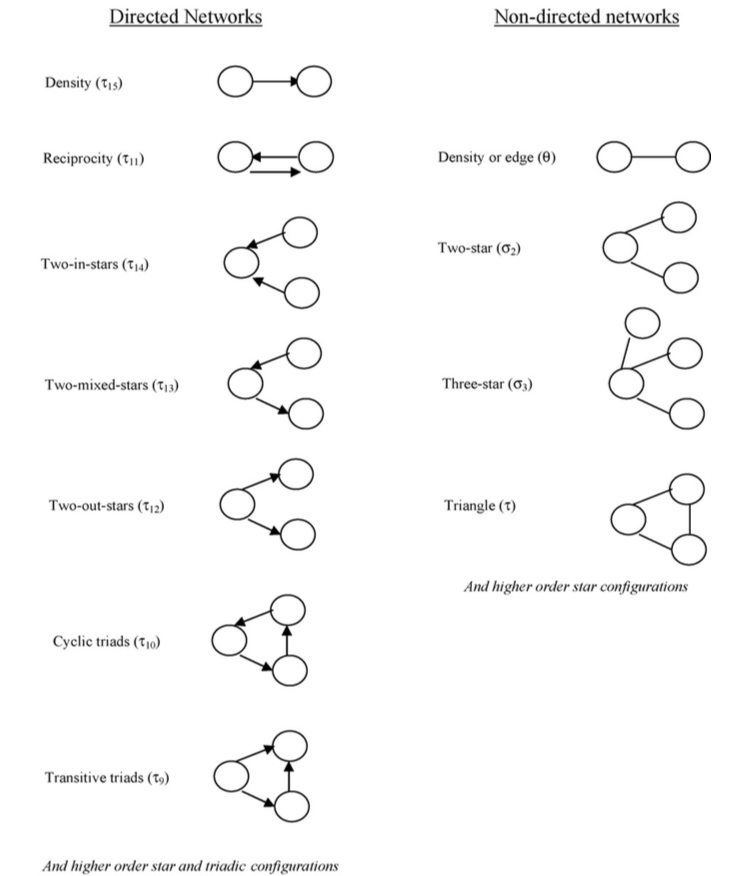
\includegraphics[height=0.8\textheight]{ergm_terms}\\
\tiny{Source: Some of the $s_k(\mathbf{y})$ endogenous network statistics \cite{Robins2007}}

\end{frame}

%------------------------------------------------


\begin{frame}
\frametitle{\insertsection}
\framesubtitle{The formulation of ERGM}

\centering
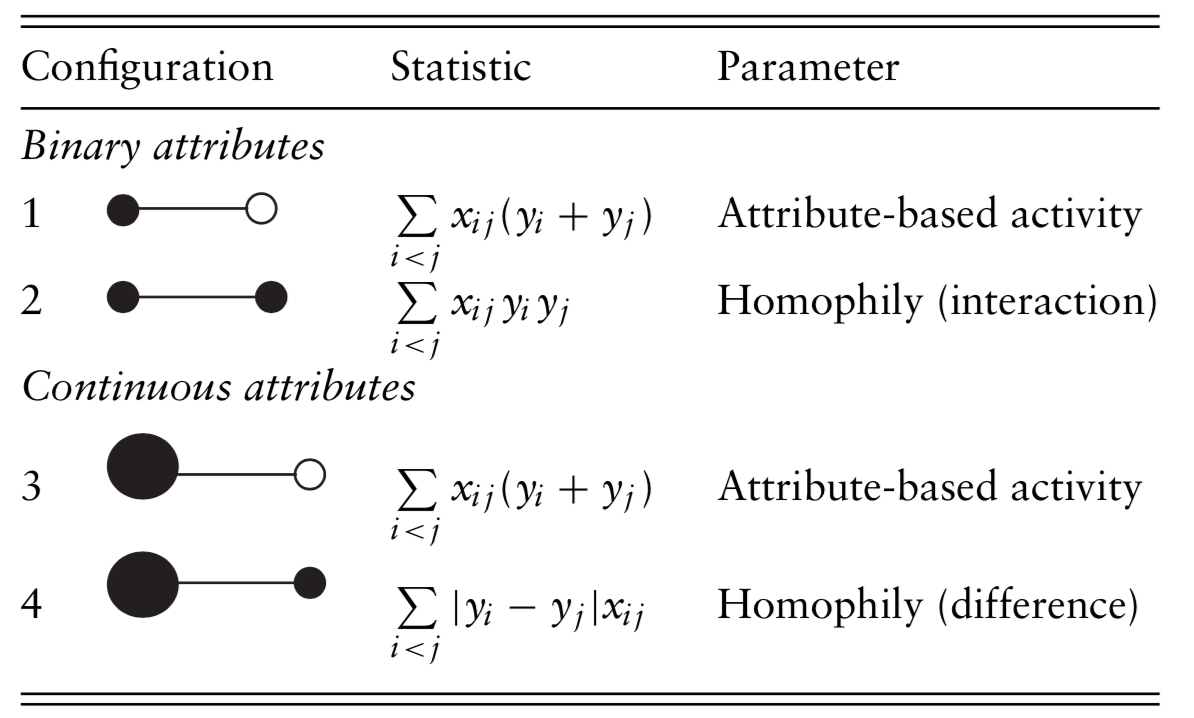
\includegraphics[height=0.5\textheight]{homophily}\\
\tiny{Source: Some of the $s_k(\mathbf{y})$ exogenous attributes \cite{Lusher2012}}

\end{frame}

%------------------------------------------------

\begin{frame}
\frametitle{\insertsection}
\framesubtitle{The formulation of ERGM}

\begin{itemize}
	\item When estimating ERGM, we try to find a vector of $\theta$ such that the network we observe in the distribution of networks is the most likely
	\item We can reformulate the ERGM as the odds of drawing the network $\mathbf{y}$ over the network $\mathbf{x}$ given $\theta$

\end{itemize}

\begin{equation*}
\frac{\mathbb{P}_\theta({\mathbf{Y} = \mathbf{y}})}{\mathbb{P}_\theta({\mathbf{Y} = \mathbf{x}})} = \frac{e^{\sum_k \theta_k s_k(\mathbf{y})}}{e^{\sum_k \theta_k s_k(\mathbf{x})}}
\end{equation*}

\begin{equation*}
\log\left(\frac{\mathbb{P}_\theta({\mathbf{Y} = \mathbf{y}})}{\mathbb{P}_\theta({\mathbf{Y} = \mathbf{x}})}\right) = \frac{\sum_k \theta_k s_k(\mathbf{y})}{\sum_k \theta_k s_k(\mathbf{x})}
\end{equation*}

\end{frame}

%------------------------------------------------

\begin{frame}
\frametitle{\insertsection}
\framesubtitle{The formulation of ERGM}

\begin{itemize}
\item If we assume $\mathbf{y}$ and $\mathbf{x}$ to differ only by one tie $y_{ij}$, we can transform the formulation as follows \cite{Hunter2008}
\end{itemize}

\begin{equation*}
logit\left(\mathbb{P}(Y_{ij} = 1 \vert \text{ n nodes}, Y_{ij}^c)\right) = \sum_k \theta_k \delta_k(\mathbf{y})
\end{equation*}

\begin{equation*}
\mathbb{P}(Y_{ij} = 1 \vert \text{ n nodes}, Y_{ij}^c) = logistic\left(\sum_k \theta_k \delta_k(\mathbf{y})\right)
\end{equation*}

\begin{itemize}
\item $\delta_k(\mathbf{y})$, change in the network statistic, i.e.\ $s_k(\mathbf{y})-s_k(\mathbf{x})$
\item when $\theta_k$ is significant the given variable $\delta_k$ play a role in generating the network
\end{itemize}

\end{frame}

%------------------------------------------------

\begin{frame}
\frametitle{\insertsection}
\framesubtitle{The formulation of ERGM}

\begin{itemize}
\item ERGM may suffer of {\color{blue}{degeneracy}}, i.e.\ the model produces that networks are fully connected or with no connections at all
\item \cite{Snijders2006, Hunter2007} proposed to include the following terms
	\begin{itemize}
	\item Geometrically Weighted Degrees (GWD)
	\item Geometrically Weighted Edgewise Shared Partnership (GWESP)
	\item Geometrically Weighted Dyadwise Shared Partnership (GWDSP)
	\end{itemize}
\item It is important you run some test (Goodness of Fit, GoF) to check that the model is generating a distribution of networks that fits your data
\end{itemize}

\end{frame}

%------------------------------------------------

\begin{frame}
\frametitle{\insertsection}
\framesubtitle{A note on econometrics}

\begin{itemize}
\item {\color{blue}{Standard statistical approaches}} (e.g.\ OLS) assume that observations are independent one of another, but this is not the case of networks where the focus is on ties between nodes (dependency) \cite{Robins2012, Snijders2011}
\medskip
\medskip
\item One observation may be associated with another through network links, thus the {\color{blue}{errors are correlated with each other}}
\medskip
\medskip
\item Example: disease contagion (sources of infection: related to the individual and network transmission of the disease)
\medskip
\medskip
\item If using regression, you should account for this effect (e.g.\ multi-level models, autocorrelation)
\end{itemize}

\end{frame}
%------------------------------------------------








%=======================================================
%	Questions
%=======================================================
\bgroup
\setbeamercolor{background canvas}{bg = orange}
\begin{frame}[plain]{}
\begin{center}
\color{white}{\Huge Questions}
\end{center}
\end{frame}
\egroup






%%=======================================================
%	Next time ...
%%=======================================================
\section*{Next time ...}
%------------------------------------------------

\bgroup
\setbeamercolor{background canvas}{bg = navyblue}
\begin{frame}[plain]{}
\begin{center}
\color{white}{\Huge\insertsection}
\end{center}
\end{frame}
\egroup

%------------------------------------------------

\begin{frame}
\frametitle{\insertsection}

\begin{itemize}

\item 	\textbf{Seminar: Network models}
	\begin{itemize}
	\item Network mathematical models in igraph
	\end{itemize}
	

\medskip
\medskip

\item 	\textbf{Lecture: Innovation networks}
	\begin{itemize}
	\item Use of network analysis to map science and technology
	\end{itemize}	

		
\end{itemize}

\end{frame}

%------------------------------------------------







%=======================================================
%	References
%=======================================================
\begin{frame}[allowframebreaks]
\frametitle{References}
\tiny
\bibliographystyle{apalike}
\bibliography{/Users/dr213/Dropbox/References/bibtex_references/library.bib}
\end{frame}
%------------------------------------------------





\end{document}